\documentclass[14pt,aspectratio=169,hyperref {pdftex,unicode},xcolor=dvipsnames]{beamer}
\usepackage[english]{babel}
\usepackage[utf8x]{inputenc}
\usepackage[T2A]{fontenc}
\usepackage{cmap}
\usepackage{qrcode}
\usepackage{booktabs}
\usepackage{paratype}
\usepackage{multicol}
\usepackage{stmaryrd}
\usepackage{mathtools}
\usepackage{mathpartir, proof}
\usepackage{amsmath, amssymb, latexsym}
\usepackage{bussproofs}
\usepackage{listingsutf8}
\usepackage[style=russian]{csquotes}
\usepackage{tikzsymbols}
\usepackage{tikz}
\usepackage{tikz-cd}
\usepackage{adjustbox}
\usepackage{color, colortbl}
\usepackage{listings}
\usepackage{bytefield}
\usepackage{xcolor}
\usepackage{graphicx}
\usepackage{fontawesome}
\usepackage{minted}
\usepackage{tcolorbox}

\usetikzlibrary{arrows.meta}
\usetikzlibrary{decorations.pathreplacing,
                positioning, 
                quotes,
                intersections,
                calc}

\newcommand{\colorbitbox}[3]{%
\rlap{\bitbox{#2}{\color{#1}\rule{\width}{\height}}}%
\bitbox{#2}{#3}}
\definecolor{lightcyan}{rgb}{0.84,1,1}
\definecolor{lightgreen}{rgb}{0.64,1,0.71}
\definecolor{lightred}{rgb}{1,0.7,0.71}
\colorlet{shadecolor}{gray!50}

\usetheme{metropolis}
\usefonttheme[]{professionalfonts}  % запрещаем beamer'у перезаписывать мат. шрифты
\metroset{numbering=fraction}
\metroset{subsectionpage=progressbar}

\setbeamercolor{frametitle}{fg=black}
\setbeamertemplate{frametitle}
{
 \vspace{3mm}\insertframetitle\par
}
\setbeamertemplate{title separator}{}
\setbeamertemplate{footnote separator}{}
%%

\DeclarePairedDelimiter\abs{\lvert}{\rvert}%
\DeclarePairedDelimiter\norm{\lVert}{\rVert}%

% Swap the definition of \abs* and \norm*, so that \abs
% and \norm resizes the size of the brackets, and the
% starred version does not.
\makeatletter
\let\oldabs\abs
\def\abs{\@ifstar{\oldabs}{\oldabs*}}
%
\let\oldnorm\norm
\def\norm{\@ifstar{\oldnorm}{\oldnorm*}}
\makeatother

\setbeamercolor{block body}{bg=mDarkTeal!30}
\setbeamercolor{block title}{bg=mDarkTeal,fg=black!2}
\setbeamerfont{block body}{shape=\upshape}

\AtBeginSection[]{
  \begin{frame}[standout]
    \insertsectionhead
  \end{frame}
}

\makeatletter
\newenvironment<>{proofs}[1][\proofname]{%
    \par
    \def\insertproofname{#1\@addpunct{.}}%
    \usebeamertemplate{proof begin}#2}
  {\usebeamertemplate{proof end}}
\newenvironment<>{proofc}{%
  \setbeamertemplate{proof begin}{\begin{block}{}}
    \par
    \usebeamertemplate{proof begin}}
  {\usebeamertemplate{proof end}}
\newenvironment<>{proofe}{%
    \par
    \pushQED{\qed}
    \setbeamertemplate{proof begin}{\begin{block}{}}
    \usebeamertemplate{proof begin}}
  {\popQED\usebeamertemplate{proof end}}
\makeatother

\addto\captionsrussian{\renewcommand*\proofname{Proof}}

\newcommand{\type}{\ensuremath{\mathtt{type}}}
\newcommand{\normal}[1]{#1 \ \mathsf{normal}}

\usepackage[dvipsnames]{xcolor}
\lstdefinelanguage{Mtt}{
  basicstyle=\ttfamily,
  comment=[l]{//},
  commentstyle={\color{gray}\ttfamily},
  identifierstyle=\color{black},
  keywords={let,letbox,in,fst,snd,box,fun,type,of,match,with,end,fix},
  keywordstyle={\color{ForestGreen}\bfseries},
  morecomment=[s]{/*}{*/},
  morestring=[b]",
  morestring=[s]{"""*}{*"""},
  ndkeywordstyle={\color{BurntOrange}\bfseries},
  sensitive=true,
  stringstyle={\color{ForestGreen}\ttfamily},
  extendedchars=false,
  inputencoding=utf8x,
  escapeinside={\%(*}{*)},
}

\newcommand{\VARIADIC}[5]{%
  \expandafter\newcommand\csname GobbleNext#1Arg\endcsname[2]{%
    \csname CheckNext#1Arg\endcsname{##1#4##2}%
    % Material moved to new argument ^^^^^^^^
  }%
  \expandafter\newcommand\csname CheckNext#1Arg\endcsname[1]{%
    \csname @ifnextchar\endcsname\bgroup{\csname GobbleNext#1Arg\endcsname{##1}}{#2{##1#5}}%
    % Wrapper macro #2 with new explicit braces ---------------------------------^-^-----^
  }%
  \expandafter\newcommand\csname #1\endcsname[2]{%
    \csname CheckNext#1Arg\endcsname{#3##1#4##2}%
    % Material moved to new argument ^^^^^^^^^^
  }%
}

\VARIADIC {llist} {\mathrm} {} {\,\,} {}
\VARIADIC {subs} {\mathrm} {[} {,\;} {]}
\def\lambdac#1#2{\lambda \mathrm{#1}. \; \mathrm{#2}}
\def\appl#1#2{\mathrm#1 \; \mathrm#2}

\tikzcdset{scale cd/.style={every label/.append style={scale=#1},
    cells={nodes={scale=#1}}}}


\newcommand*\circled[1]{\tikz[baseline=(char.base)]{
  \node[shape=circle,draw,inner sep=2pt] (char) {#1};}}

\newenvironment{keypoints}{
  \begin{itemize}
      \setlength{\itemsep}{6pt}
      \setlength{\leftskip}{10pt}
      \setbeamertemplate{itemize item}{\faLightbulbO}
      \setbeamercolor{item}{fg=black,bg=yellow!20}
  }
  {
  \end{itemize}
}

\newenvironment{questions}{
  \begin{itemize}
      \setlength{\itemsep}{6pt}
      \setlength{\leftskip}{10pt}
      \setbeamertemplate{itemize item}{\faQuestion}
      \setbeamercolor{item}{fg=black,bg=yellow!20}
  }
  {
  \end{itemize}
}

\renewenvironment{examples}{
  \begin{itemize}
      \setlength{\itemsep}{6pt}
      \setlength{\leftskip}{10pt}
      \setbeamertemplate{itemize item}{\faPencil}
      \setbeamercolor{item}{fg=black,bg=yellow!20}
  }
  {
  \end{itemize}
}

\tcbuselibrary{skins}
\tcbset{
    mygraphicbox/.style={
        colback=white,
        colframe=mDarkTeal,
        fonttitle=\bfseries,
        boxrule=0.5mm,
        arc=4mm,
        width=\textwidth,
        boxsep=4pt,
        left=4pt,
        right=4pt,
        top=6pt,
        bottom=6pt
    }
}

\begin{document}

\begin{frame}[plain]
  \begin{center}
    {\Large\textbf{Repairik: Code Repairing with LLMs}}

    Andrei Kozyrev, Nikita Khramov, Ivan Kabashnyi

    December 2024
  \end{center}
\end{frame}

\section{Overview}

\begin{frame}
  \frametitle{Setting}

  \begin{keypoints}
    \item Code interpretation can be time-consuming for big amount of code
    \item The ability of small-sized models to find errors is low
    \item The good model-based interpreter can be used for program repair    
  \end{keypoints}
\end{frame}

\begin{frame}
  \frametitle{Contributions}

  \begin{keypoints}
    \item Pipeline for dataset generation
    \item Dataset for error prediction
    \item Fine-tuned model for error prediction    
  \end{keypoints}
\end{frame}

\section{Dataset}

\begin{frame}
  \frametitle{LiveCodeBench}

  \begin{keypoints}
    \item A benchmark for evaluating large language models (LLMs) on code generation tasks.
    \item Designed to be ``contamination-free''
    \item Continuously updated with new problems (from LeetCode, CodeForces and etc.)
    \item Provides a holistic evaluation
    \item Specifically contains problem statements and tests    
  \end{keypoints}
  
\end{frame}


\begin{frame}
  \frametitle{Data Generation Pipeline}

\begin{center}
    \scalebox{0.76}{
      \begin{tikzpicture}[
        node distance=2cm and 2.5cm,
        every node/.style={draw, rounded corners, minimum height=1cm, minimum width=2.5cm, align=center, font=\sffamily,font=\footnotesize},
        every path/.style={-Stealth, thick}
        ]
        
        % Nodes
        \node[fill=green!10] (livecodebench) {LiveCodeBench};
        \node[right=of livecodebench, fill=green!10] (llmgen) {LLM-generation};
        \node[right=of llmgen, fill=green!10] (llmclass) {LLM-classification};
        \node[below=of llmclass, fill=green!10] (executor) {Python Executor};
        \node[above right=of llmclass, fill=green!10] (repairik) {Repairik Dataset};
        
        % Arrows
        \draw (livecodebench) -- node[midway, draw=none] {Prompt + \\ Statement} (llmgen);
        \draw (llmgen) -- node[midway, draw=none] {Gen. Solution \\ + Prompt} (llmclass);
        \draw[bend left=10] (llmgen) to node[right, draw=none] {Gen. Solution} (executor);
        \draw[bend left=10] (executor) to node[left, draw=none] {Gen. Solution} (llmgen);
        \draw[bend right=15] (livecodebench) to node[left, draw=none] {Tests} (executor);
        \draw (llmgen) -- node[draw=none, sloped, above] {Gen. Solution} (repairik);
        \draw (llmclass) -- node[midway, draw=none, sloped] {Predicted error \\ or not found} (repairik);
        \draw (executor) -- node[midway, draw=none, sloped, below] {Ground Truth Error \\ or Success} (repairik);
        
        \end{tikzpicture}
    }
\end{center}

  % \begin{tcolorbox}[mygraphicbox, title=Data Generation Pipeline]
  %   \begin{center}
  %       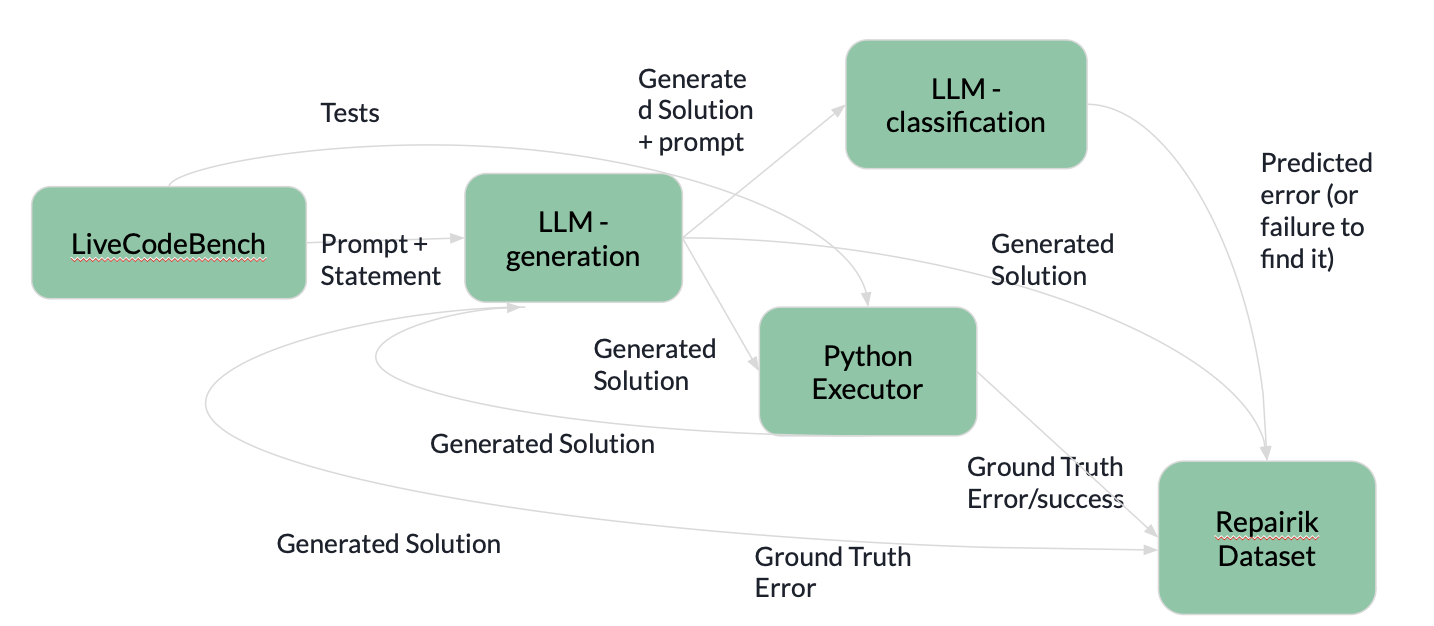
\includegraphics[width=0.8\textwidth]{images/pipeline.png}
  %   \end{center}
  % \end{tcolorbox}
  
\end{frame}

\begin{frame}
  \frametitle{Program Generation \& Repair Ability}

  Models: \textbf{Anthropic Claude} 2 and \textbf{Llama 3 Instruct 8B}
  
  LiveCodeBench: 706 problems

  {\footnotesize
  \begin{multicols}{2}
    \textbf{Llama 3 (was run on 706 problems):}
    \begin{itemize}
      \item Generated samples with predictable error (not WA or TL): 84
      \item Generated correct samples: 103
      \begin{itemize}
        \item {\footnotesize after repair: 3 }
      \end{itemize}
    \end{itemize}
    \columnbreak
    \textbf{Anthropic Claude 2 (on 521 problems):}
    \begin{itemize}
      \item Generated samples with predictable error (not WA or TL): 171
      \item Generated correct samples: 118
      \begin{itemize}
        \item {\footnotesize after repair: 2 }
      \end{itemize}
    \end{itemize}
  \end{multicols}}
  
\end{frame}

\begin{frame}
  \frametitle{Program Generation \& Repair Ability}

  {\footnotesize
  \begin{multicols}{2}
    \textbf{Llama 3 (was run on 706 problems):}
    \begin{itemize}
      { \color{shadecolor}
      \item Generated samples with predictable error (not WA or TL): 84
      \item Generated correct samples: 103
      \begin{itemize}
        \item {\footnotesize \color{shadecolor} after repair: 3}
      \end{itemize} }
      \item Samples with predicted error: 53
      \begin{itemize}
        \item {\footnotesize correctly classified error type: 3 }
      \end{itemize}
    \end{itemize}
    \columnbreak{}
    \textbf{Anthropic Claude 2 (on 521 problems):}
    \begin{itemize}
      { \color{shadecolor}
      \item Generated samples with predictable error (not WA or TL): 171
      \item Generated correct samples: 118
      \begin{itemize}
        \item {\footnotesize \color{shadecolor} after repair: 2 }
      \end{itemize} }
      \item Samples with predicted error: 15
      \begin{itemize}
        \item {\footnotesize correctly classified error type: 8 }
      \end{itemize}
    \end{itemize}
  \end{multicols}}
\end{frame}

\begin{frame}
  \frametitle{Dataset Statistics}

  \begin{tcolorbox}[mygraphicbox, title=Entries per result]
    \begin{center}
        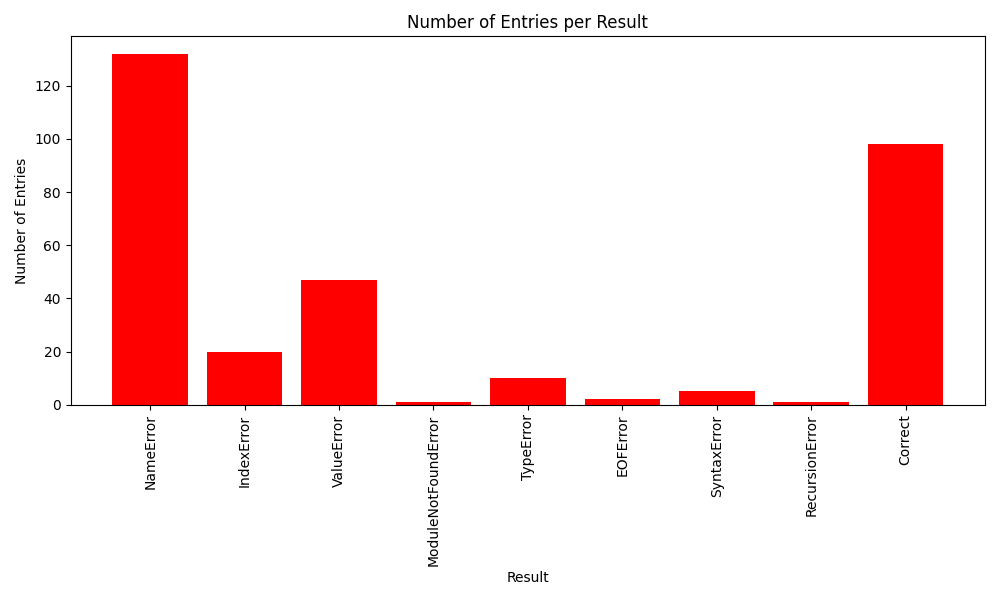
\includegraphics[width=0.55\textwidth]{images/entries_per_result_natural.png}
    \end{center}
  \end{tcolorbox}
\end{frame}

\begin{frame}
  \frametitle{Dataset After Augmentation}

  \begin{tcolorbox}[mygraphicbox, title=Entries per result: Augmented]
    \begin{center}
        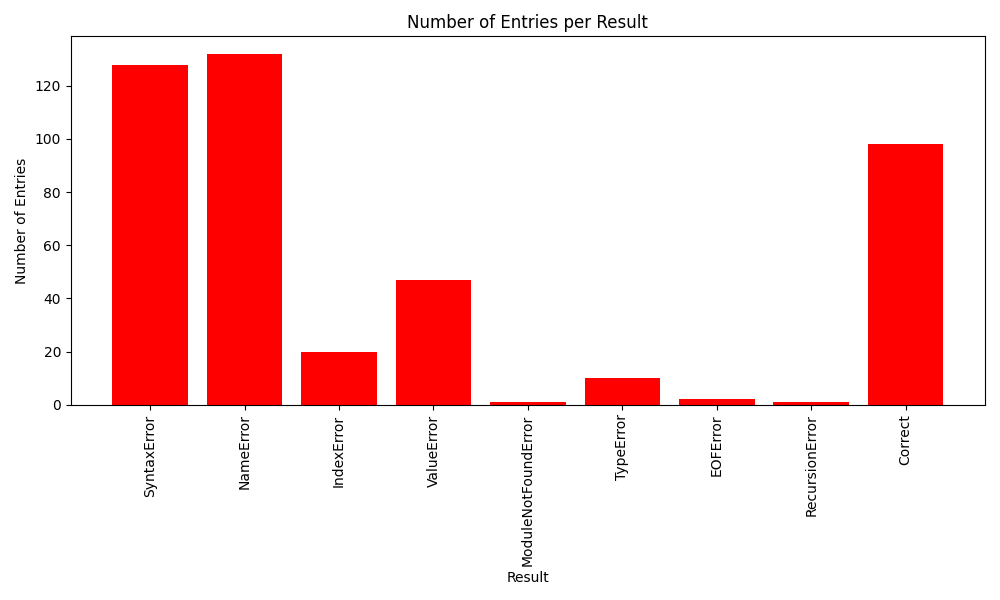
\includegraphics[width=0.55\textwidth]{images/entries_per_result.png}
    \end{center}
  \end{tcolorbox}

\end{frame}

\section{Model Tuning}

\begin{frame}
  \frametitle{Data Generation Pipeline}

\begin{center}
    \scalebox{0.76}{
      \begin{tikzpicture}[
        node distance=2cm and 2.5cm,
        every node/.style={draw, rounded corners, minimum height=1cm, minimum width=2.5cm, align=center, font=\sffamily,font=\footnotesize},
        every path/.style={-Stealth, thick}
        ]
        
        % Nodes
        \node[fill=green!10] (livecodebench) {LiveCodeBench};
        \node[right=of livecodebench, fill=green!10] (llmgen) {LLM-generation};
        \node[right=of llmgen, fill=green!10] (llmclass) {LLM-classification};
        \node[below=of llmclass, fill=red!10] (executor) {Emulated Executor};
        \node[above right=of llmclass, fill=green!10] (repairik) {Repairik Dataset};
        
        % Arrows
        \draw (livecodebench) -- node[midway, draw=none] {Prompt + \\ Statement} (llmgen);
        \draw (llmgen) -- node[midway, draw=none] {Gen. Solution \\ + Prompt} (llmclass);
        \draw[bend left=10] (llmgen) to node[right, draw=none] {Gen. Solution} (executor);
        \draw[bend left=10] (executor) to node[left, draw=none] {Gen. Solution} (llmgen);
        \draw[bend right=15] (livecodebench) to node[left, draw=none] {Tests} (executor);
        \draw (llmgen) -- node[draw=none, sloped, above] {Gen. Solution} (repairik);
        \draw (llmclass) -- node[midway, draw=none, sloped] {Predicted error \\ or not found} (repairik);
        \draw (executor) -- node[midway, draw=none, sloped, below] {Ground Truth Error \\ or Success} (repairik);
        
        \end{tikzpicture}
    }
\end{center}
  
\end{frame}

\begin{frame}
  \frametitle{Emulating Executor}

\begin{center}
    \scalebox{0.76}{
      \begin{tikzpicture}[
        node distance=2cm and 1.45cm,
        every node/.style={draw, rounded corners, minimum height=1cm, minimum width=2.5cm, align=center, font=\sffamily,font=\footnotesize},
        every path/.style={-Stealth, thick}
        ]
        
        % Nodes
        \node[fill=green!10] (llmgen) {LLM-generation};
        \node[right=of llmgen, fill=red!10] (binerror) {Binary Error prediction};
        \node[right=of binerror, fill=red!10] (errclass) {Error classification};
        \node[right=of errclass, fill=green!10] (coderep) {Code repair from diagnostic};
        \node[below=of errclass, fill=green!30] (output) {Output};
        
        % Arrows
        \draw (llmgen) -- (binerror);
        \draw (binerror) -- (errclass);
        \draw (errclass) -- (coderep);
        \draw (binerror) -- (output);
        \draw (coderep) -- (output);
        
        \end{tikzpicture}
    }
\end{center}
  
\end{frame}

\begin{frame}[fragile]
  \frametitle{Binary Error Classifier}

  \begin{table}[ht]
    \centering
    \begin{tabular}{ll}
      \toprule
      \textbf{Model} & \textbf{Accuracy} \\
      \midrule
      Llama before fine-tuning & 0.48 \\
      Roberta full fine-tuning & 0.52 \\
      Roberta LoRa fine-tuning & 0.75 \\
      Llama LoRa fine-tuning & 0.70 \\
      \bottomrule
    \end{tabular}
    \caption{Model accuracy comparison}
  \end{table}
  
\end{frame}

\begin{frame}[fragile]
  \frametitle{Binary Error Classifier}

  \begin{multicols}{2}
    \begin{keypoints}
      \item 6 epochs
      \item 5e-4 learning rate
      \item Batch size 8
    \end{keypoints}
    \columnbreak{}
    \begin{keypoints}
      \item LoRa rank 16
      \item LoRa alpha 16
      \item LoRa dropout 0.05
    \end{keypoints}
  \end{multicols}
  
\end{frame}

\begin{frame}
  \frametitle{Dataset}

  \begin{tcolorbox}[mygraphicbox, title=Error Labels Distribution]
    \begin{center}
        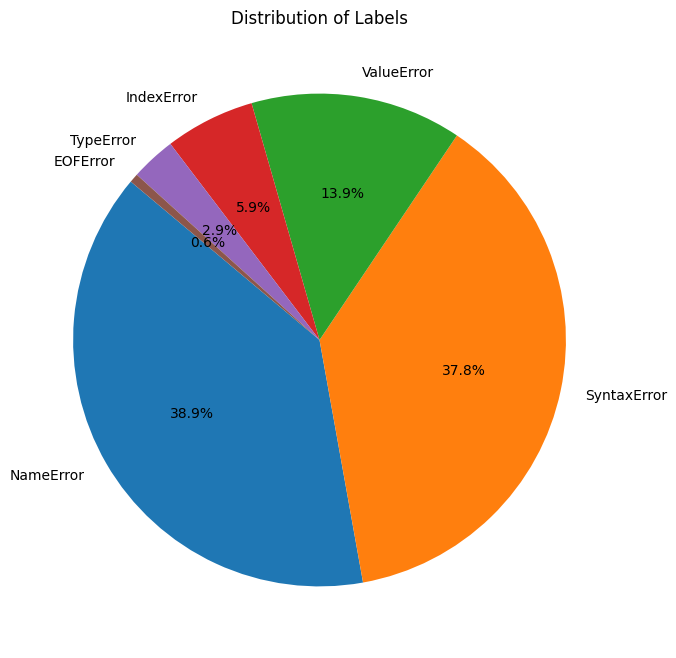
\includegraphics[width=0.35\textwidth]{images/dataset_dist.png}
    \end{center}
  \end{tcolorbox}
  
\end{frame}

\begin{frame}[fragile]
  \frametitle{Multiclass Error Classifier}

  \begin{multicols}{2}
    \begin{keypoints}
      \item 6 epochs
      \item 5e-4 learning rate
      \item Batch size 8
    \end{keypoints}
    \columnbreak{}
    \begin{keypoints}
      \item LoRa rank 16
      \item LoRa alpha 16
      \item LoRa dropout 0.05
    \end{keypoints}
  \end{multicols}

  \begin{keypoints}
    \item Use weighted Cross Entropy due to unbalanced dataset 
    \item Llama checkpoint – \texttt{codellama/CodeLlama-7b-hf}
  \end{keypoints}
  
\end{frame}

\begin{frame}[fragile]
  \frametitle{Multiclass Error Classifier}

  \begin{center}
    {\footnotesize
    \begin{table}[ht]
      \centering
      \begin{tabular}{c c c c c c}
      \toprule
      \textbf{Epoch} & \textbf{Training Loss} & \textbf{Precision} & \textbf{Recall} & \textbf{F1-score} & \textbf{Accuracy} \\ \midrule
      1              & 1.08                   & 0.58               & 0.59            & 0.56              & 0.59              \\ \midrule
      2              & 0.75                   & 0.76               & 0.73            & 0.74              & 0.73              \\ \midrule
      3              & 0.75                   & 0.72               & 0.71            & 0.68              & 0.71              \\ \midrule
      4              & 0.81                   & 0.75               & 0.75            & 0.74              & 0.75              \\ \midrule
      5              & 0.28                   & 0.77               & 0.75            & 0.76              & 0.75              \\ \midrule
      6              & 0.43                   & 0.85               & 0.78            & 0.82              & 0.78              \\ \bottomrule
      \end{tabular}
      \caption{Metrics across epochs with 2-decimal precision.}\label{tab:metrics}
    \end{table} }
  \end{center}
  
\end{frame}


\begin{frame}[fragile]
  \frametitle{Multiclass Error Classifier}

  \begin{tcolorbox}[mygraphicbox, title=Emulating Executor]
    \begin{center}
        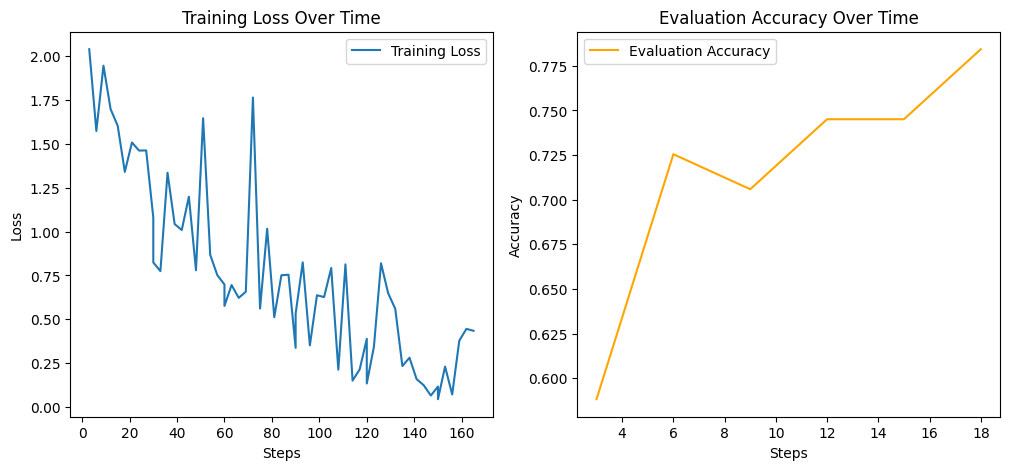
\includegraphics[width=0.7\textwidth]{images/metrics_multiclass.png}
    \end{center}
  \end{tcolorbox}
  
\end{frame}

\begin{frame}[fragile]
  \frametitle{Conclusion}

  \begin{keypoints}
      \item Repairing generated code from execution feedback doesn't show much improvement for small models
      \item The ability of a small fine-tuned model to classify errors (even with a small amount of data) seems promising
      \item Validation of code generated by LLM requires substantial engineering efforts
  \end{keypoints}
  
\end{frame}

\begin{frame}[fragile]
  \frametitle{Conclusion}

  \begin{examples}
      \item Pipeline for dataset generation
      \item Small dataset for code repairing task
      \item Fine-tuned model for error prediction
  \end{examples}
  
\end{frame}

\section{Thank you!} 

\end{document}
